\documentclass[11pt,a4paper]{article}
% ===========================================================================
%  Polycopié de prérequis — Comptabilité prudentielle (M2 alternance)
%  Préambule partagé
%  F. Borel-Mathurin — Université Paris 1 Panthéon-Sorbonne
% ===========================================================================

\usepackage[utf8]{inputenc}
\usepackage[T1]{fontenc}
\IfFileExists{french.ldf}{\usepackage[french]{babel}}{}
\IfFileExists{lmodern.sty}{\usepackage{lmodern}}{}
\usepackage[a4paper,margin=2.4cm]{geometry}

\usepackage{amsmath,amssymb}
\usepackage{booktabs}
\usepackage{array}
\usepackage{enumitem}
\usepackage{xcolor}
\usepackage{tcolorbox}
\tcbuselibrary{skins,breakable}
\usepackage{tikz}
\usetikzlibrary{arrows.meta,positioning,calc}
\usepackage{fancyhdr}
\usepackage[hidelinks]{hyperref}
\usepackage{makeidx}
\makeindex
\IfFileExists{eurosym.sty}{\usepackage{eurosym}}{\providecommand{\euro}{\texteuro}}

% ---------------------------------------------------------------- couleurs
% À remplacer par les valeurs exactes de la charte si besoin.
\definecolor{bleuactu}{RGB}{0,84,150}
\definecolor{vertactu}{RGB}{0,132,100}
\definecolor{rougeactu}{RGB}{175,30,45}
\definecolor{orangeactu}{RGB}{230,140,0}
\definecolor{grisactu}{RGB}{110,110,110}

% ------------------------------------------------- version étudiant/corrigé
% \correctiontrue  -> corrigés inclus
% \correctionfalse -> version étudiant
\newif\ifcorrection
\correctiontrue

% ------------------------------------------------------------------ boîtes
\newtcolorbox{notion}[1]{%
  breakable, enhanced, colback=bleuactu!4, colframe=bleuactu,
  boxrule=0.4pt, left=8pt, right=8pt, top=6pt, bottom=6pt,
  fonttitle=\bfseries\sffamily, coltitle=white, title={#1}}

\newtcolorbox{generalisation}[1]{%
  breakable, enhanced, colback=orangeactu!5, colframe=orangeactu!85!black,
  boxrule=0.4pt, left=8pt, right=8pt, top=6pt, bottom=6pt,
  fonttitle=\bfseries\sffamily, coltitle=white, title={#1}}

\newtcolorbox{pont}[1]{%
  breakable, enhanced, colback=rougeactu!4, colframe=rougeactu,
  boxrule=0.4pt, left=8pt, right=8pt, top=6pt, bottom=6pt,
  fonttitle=\bfseries\sffamily, coltitle=white, title={#1}}

\newtcolorbox{refreg}{%
  breakable, enhanced, colback=grisactu!6, colframe=grisactu!60,
  boxrule=0.4pt, left=8pt, right=8pt, top=6pt, bottom=6pt,
  fontupper=\small}

% --------------------------------------------------------------- exercices
\newcounter{exo}[section]
\renewcommand{\theexo}{\thesection.\arabic{exo}}

\newenvironment{exercice}[1][]{%
  \refstepcounter{exo}%
  \par\medskip\noindent
  \begin{tcolorbox}[breakable, enhanced, colback=white, colframe=vertactu,
     boxrule=0.4pt, left=8pt, right=8pt, top=6pt, bottom=6pt,
     fonttitle=\bfseries\sffamily, coltitle=white,
     title={Exercice \theexo\ifx\relax#1\relax\else\ --- #1\fi}]}%
  {\end{tcolorbox}\par\medskip}

\newenvironment{corrige}{%
  \ifcorrection
    \par\smallskip\noindent
    \begin{tcolorbox}[breakable, enhanced, colback=vertactu!4,
       colframe=vertactu!50, boxrule=0.4pt, left=8pt, right=8pt,
       top=6pt, bottom=6pt, fontupper=\small,
       title={\itshape Corrigé}, fonttitle=\small\itshape,
       coltitle=vertactu!80!black, colbacktitle=vertactu!10]%
  \else
    \setbox0\vbox\bgroup
  \fi}%
  {\ifcorrection\end{tcolorbox}\par\smallskip\else\egroup\fi}

% ------------------------------------------------------------- échéanciers
\tikzset{
  timeaxis/.style={-{Latex[length=2mm]}, thick, grisactu},
  timenode/.style={circle, fill=bleuactu, inner sep=1.1pt},
  flux/.style={-{Latex[length=2mm]}, thick, vertactu},
  fluxneg/.style={-{Latex[length=2mm]}, thick, rougeactu},
  etiq/.style={font=\scriptsize, inner sep=1pt}
}

% ------------------------------------------------------------------ titres
\usepackage{titlesec}
\titleformat{\section}{\Large\bfseries\sffamily\color{bleuactu}}{\thesection}{0.7em}{}
\titleformat{\subsection}{\large\bfseries\sffamily\color{bleuactu!80!black}}{\thesubsection}{0.6em}{}

\pagestyle{fancy}
\fancyhf{}
\fancyhead[L]{\small\sffamily\color{grisactu}Prérequis --- Comptabilité prudentielle}
\fancyhead[R]{\small\sffamily\color{grisactu}\thepage}
\renewcommand{\headrulewidth}{0.2pt}

\newcommand{\notation}[2]{\item[{$#1$}] #2}  % accolades : #1 peut contenir des crochets


% Version étudiant par défaut ; `make pdf` produit aussi la version corrigée
% (prerequis-corrige.pdf) en définissant \Corrige avant la compilation.
\ifdefined\Corrige\correctiontrue\else\correctionfalse\fi

\title{\vspace{-1.5cm}\sffamily\bfseries\color{bleuactu}
       Prérequis de comptabilité prudentielle\\[2mm]
       \large\mdseries\color{black}Rappels et exercices corrigés}
\author{\sffamily Fabrice Borel-Mathurin \\+ crew}
\date{\sffamily\small Université Paris 1 Panthéon-Sorbonne \\ Master 2 en alternance}

\begin{document}
\maketitle
\thispagestyle{empty}

\begin{center}
\begin{minipage}{0.86\textwidth}
\small
Ce polycopié se parcourt dans l'ordre. Chaque unité reprend la précédente et lui
ajoute un seul ingrédient : plusieurs dates, puis la dépendance aux taux, puis
l'aléa, puis l'optionalité. Au terme de cette progression, le calcul d'une
meilleure estimation n'est plus qu'un cas particulier de la toute première
formule.

\medskip
Chaque unité suit la même trame --- une notion, un exercice d'application, la
généralisation de la notion, des exercices plus complexes --- et se termine par
le lien explicite avec le dispositif Solvabilité~II et les références
réglementaires correspondantes.
\end{minipage}
\end{center}

\vspace{6mm}
\tableofcontents
\newpage

\section{Un flux certain}
\label{sec:U1}

Toute la comptabilité prudentielle repose sur une seule opération, répétée et
généralisée : ramener à aujourd'hui la valeur d'un montant disponible plus tard.
Cette unité en pose la forme la plus simple. Les cinq suivantes ne feront
qu'y ajouter, une par une, les complications du monde réel.

\subsection{La notion : valeur actuelle d'un flux unique}

\begin{notion}{Actualisation et capitalisation}
Un montant $C$ disponible dans $n$ années n'a pas la même valeur qu'un montant
$C$ disponible aujourd'hui. Au taux annuel $r$, un euro placé aujourd'hui vaut
$(1+r)^n$ euros dans $n$ ans : c'est la \emph{capitalisation}\index{capitalisation}.

L'opération inverse, l'\emph{actualisation}\index{actualisation}, ramène un flux
futur à sa valeur d'aujourd'hui :
\[
  V_0 \;=\; \frac{C}{(1+r)^n} \;=\; C \times v^{\,n},
  \qquad\text{avec}\qquad v \;=\; \frac{1}{1+r}.
\]
Le terme $v^{\,n}$ est le \emph{facteur d'actualisation}\index{facteur d'actualisation}
à l'horizon $n$. Il est toujours compris entre $0$ et $1$ dès que $r>0$.
\end{notion}

Deux propriétés doivent devenir des réflexes, car elles se retrouveront à chaque
étage de la progression : la valeur actuelle \emph{décroît} quand le taux
augmente, et elle \emph{décroît} quand l'échéance s'éloigne.

\begin{center}
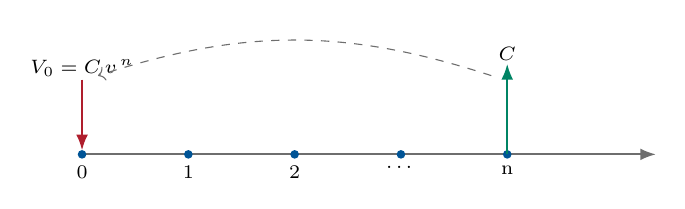
\begin{tikzpicture}[x=1.35cm, y=1cm]
  \draw[timeaxis] (0,0) -- (5.4,0);
  \foreach \x/\l in {0/0, 1/1, 2/2, 3/{\dots}, 4/n}
    { \node[timenode] at (\x,0) {}; \node[etiq, below=3pt] at (\x,0) {\l}; }
  \draw[flux] (4,0) -- (4,1.15);
  \node[etiq, above] at (4,1.15) {$C$};
  \draw[fluxneg] (0,0.95) -- (0,0.05);
  \node[etiq, above] at (0,0.95) {$V_0 = C\,v^{\,n}$};
  \draw[->, dashed, grisactu] (3.85,1.0) to[bend right=18] (0.15,1.0);
\end{tikzpicture}
\end{center}

\begin{exercice}[valeur actuelle]
Un flux certain de $25\,000$~\euro{} sera perçu dans $7$~ans. Le taux
d'actualisation annuel est de $3{,}20\,\%$. Calculer sa valeur actuelle.
\end{exercice}

\begin{corrige}
\[
  V_0 = \frac{25\,000}{(1{,}032)^{7}} = \frac{25\,000}{1{,}24669} \approx 20\,053\ \text{\euro}.
\]
Autrement dit, disposer de $20\,053$~\euro{} aujourd'hui équivaut à disposer de
$25\,000$~\euro{} dans sept ans, si l'on peut placer son argent à $3{,}20\,\%$.
\end{corrige}

\begin{exercice}[capitalisation]
Un capital de $15\,000$~\euro{} est placé pendant $12$~ans au taux annuel de
$2{,}50\,\%$. Quel montant sera disponible au terme ?
\end{exercice}

\begin{corrige}
\[
  C_{12} = 15\,000 \times (1{,}025)^{12} = 15\,000 \times 1{,}34489 \approx 20\,173\ \text{\euro}.
\]
C'est l'opération réciproque de la précédente : on multiplie au lieu de diviser.
\end{corrige}

\subsection{Généralisation : les conventions de taux}

\begin{generalisation}{Un taux n'a de sens qu'avec sa convention}
Annoncer « $4\,\%$ » ne suffit pas. Il faut préciser la périodicité de
capitalisation et la règle de comptage des jours. Deux distinctions suffisent
pour la suite du cours.

\medskip
\textbf{Taux proportionnel et taux équivalent.} Pour passer d'un taux annuel
$r$ à un taux sur une fraction $1/k$ d'année, deux conventions coexistent :
\[
  \underbrace{r^{\text{prop}}_{k} = \frac{r}{k}}_{\text{proportionnel}}
  \qquad\text{et}\qquad
  \underbrace{r^{\text{éq}}_{k} = (1+r)^{1/k} - 1}_{\text{équivalent}}.
\]
Seul le taux équivalent respecte la capitalisation : $(1+r^{\text{éq}}_{k})^{k} = 1+r$.
Le taux proportionnel, lui, surestime toujours le rendement réel.

\medskip
\textbf{Base de calcul des jours.} /!\ Attention /!\ La convention des marché monétaire est que pour les durées inférieures à un an, on n’utilise pas l’actualisation pour le calcul des intérêts courus, mais la formule suivante : 
\[
  I = C \times r \times \frac{\text{nombre de jours}}{\text{base}}.
\]
La base de calcul des jours peut être de $360$ ou $365$ jours : \emph{exact/360}\index{exact/360} (base monétaire) ou \emph{exact/365}\index{exact/365} (base obligataire) ; la base $360$ produit mécaniquement des intérêts plus élevés que la base $365$ pour un même taux affiché.
\end{generalisation}

\begin{exercice}[proportionnel contre équivalent]
Le taux annuel est de $4{,}00\,\%$. Calculer le taux semestriel proportionnel et
le taux semestriel équivalent. Un capital de $200\,000$~\euro{} est placé un an,
avec capitalisation semestrielle : chiffrer l'écart entre les deux conventions.
\end{exercice}

\begin{corrige}
Taux proportionnel : $r^{\text{prop}}_{2} = 4{,}00/2 = 2{,}0000\,\%$.

Taux équivalent : $r^{\text{éq}}_{2} = (1{,}04)^{1/2} - 1 = 1{,}98039\,\%$.

\medskip
Au bout d'un an, soit deux semestres :
\begin{align*}
  \text{convention proportionnelle} &: 200\,000 \times (1{,}02)^{2} = 208\,080{,}00\ \text{\euro} \\
  \text{convention équivalente}     &: 200\,000 \times (1{,}04)\phantom{^{2}} = 208\,000{,}00\ \text{\euro}
\end{align*}
L'écart est de $80$~\euro{} sur un an. Il paraît anodin ; rapporté à un
portefeuille de provisions techniques de plusieurs centaines de millions et à un
horizon de projection de trente ans, il ne l'est plus.
\end{corrige}

\begin{exercice}[bases de calcul]
Un placement de $500\,000$~\euro{} est effectué pour $91$~jours au taux de
$3{,}00\,\%$. Calculer les intérêts en base exact/360 puis en base exact/365, et
commenter l'écart.
\end{exercice}

\begin{corrige}
\begin{align*}
  \text{exact}/360 &: 500\,000 \times 0{,}03 \times \tfrac{91}{360} = 3\,791{,}67\ \text{\euro} \\
  \text{exact}/365 &: 500\,000 \times 0{,}03 \times \tfrac{91}{365} = 3\,739{,}73\ \text{\euro}
\end{align*}
L'écart atteint $51{,}94$~\euro, soit $1{,}39\,\%$ des intérêts. Le rapport des
deux bases vaut exactement $365/360$, quel que soit le montant, le taux ou la
durée : c'est un écart de convention, pas un écart économique.
\end{corrige}

\begin{pont}{Où cela sert dans Solvabilité~II}
Le facteur $v^{\,n}$ de cette unité est très exactement celui qui sera appliqué
à chaque flux de prestation dans le calcul de la meilleure estimation. La seule
différence, à ce stade purement technique, est que le taux $r$ n'y est pas choisi
librement : il est lu sur la courbe des taux sans risque publiée chaque mois par
l'EIOPA, et il varie selon l'échéance du flux. C'est l'objet de l'unité~3.
\end{pont}

\begin{refreg}
\textbf{Références.} Directive 2009/138/CE, article~77, paragraphe~2 : la
meilleure estimation est la moyenne pondérée des flux de trésorerie futurs
compte tenu de la valeur temporelle de l'argent, obtenue au moyen de la courbe
des taux sans risque pertinente. \\
Les structures par terme sans risque sont publiées mensuellement par l'EIOPA,
accompagnées de leur documentation technique.
\end{refreg}

\subsection*{Notations introduites}
\begin{description}[leftmargin=3cm, style=nextline, font=\normalfont]
  \notation{C}{montant nominal d'un flux}
  \notation{r}{taux d'actualisation annuel}
  \notation{n}{horizon, en années}
  \notation{v = (1+r)^{-1}}{facteur d'actualisation à un an}
  \notation{V_0}{valeur actuelle}
\end{description}

\newpage
\section{Un échéancier certain}
\label{sec:U2}

L'unité précédente traitait un flux isolé. On ajoute ici le premier ingrédient :
\emph{plusieurs dates}. Rien de conceptuellement neuf --- on additionne des
valeurs actuelles --- mais cette addition est la forme sous laquelle se
présentent la quasi-totalité des engagements d'assurance.

\subsection{La notion : valeur actuelle nette d'un échéancier}

\begin{notion}{Sommer des flux actualisés}
Un \emph{échéancier}\index{échéancier} est une suite de flux $(C_1,\dots,C_n)$
associés à des dates $(t_1,\dots,t_n)$. Sa valeur actuelle est la somme des
valeurs actuelles de chaque flux :
\[
  V_0 \;=\; \sum_{k=1}^{n} \frac{C_k}{(1+r)^{t_k}}.
\]
Lorsque l'échéancier comprend un décaissement initial $C_0$, on parle de
\emph{valeur actuelle nette}\index{valeur actuelle nette} :
\[
  \mathrm{VAN} \;=\; -\,C_0 \;+\; \sum_{k=1}^{n} \frac{C_k}{(1+r)^{t_k}}.
\]
Une opération est créatrice de valeur si sa VAN est positive.
\end{notion}

Deux conventions doivent être fixées avant tout calcul, et elles le seront de
même dans les projections prudentielles : les flux sont-ils supposés survenir en
début ou en fin de période, et le taux est-il constant sur tout l'horizon ? Sauf
mention contraire, on retient ici des flux de fin de période et un taux constant.

\begin{center}
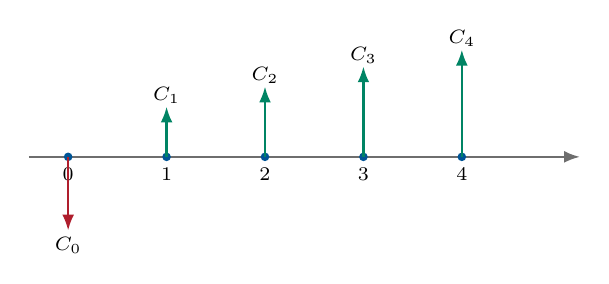
\begin{tikzpicture}[x=1.25cm, y=0.85cm]
  \draw[timeaxis] (-0.4,0) -- (5.2,0);
  \foreach \x/\l in {0/0, 1/1, 2/2, 3/3, 4/4}
    { \node[timenode] at (\x,0) {}; \node[etiq, below=3pt] at (\x,0) {\l}; }
  \draw[fluxneg] (0,0) -- (0,-1.1);
  \node[etiq, below] at (0,-1.15) {$C_0$};
  \draw[flux] (1,0) -- (1,0.75); \node[etiq, above] at (1,0.75) {$C_1$};
  \draw[flux] (2,0) -- (2,1.05); \node[etiq, above] at (2,1.05) {$C_2$};
  \draw[flux] (3,0) -- (3,1.35); \node[etiq, above] at (3,1.35) {$C_3$};
  \draw[flux] (4,0) -- (4,1.6);  \node[etiq, above] at (4,1.6)  {$C_4$};
\end{tikzpicture}
\end{center}

\begin{exercice}[valeur actuelle d'un échéancier]
Un projet génère les flux suivants, en fin d'année : $12\,000$~\euro,
$15\,000$~\euro, $18\,000$~\euro{} et $20\,000$~\euro. Le taux d'actualisation
est de $3{,}50\,\%$. Calculer la valeur actuelle de cet échéancier.
\end{exercice}

\begin{corrige}
\begin{center}\small
\begin{tabular}{ccrr}
\toprule
Année & Flux & Facteur $v^{k}$ & Flux actualisé \\
\midrule
1 & $12\,000$ & $0{,}96618$ & $11\,594{,}20$ \\
2 & $15\,000$ & $0{,}93351$ & $14\,002{,}33$ \\
3 & $18\,000$ & $0{,}90194$ & $16\,234{,}86$ \\
4 & $20\,000$ & $0{,}87144$ & $17\,428{,}84$ \\
\midrule
\multicolumn{3}{r}{\textbf{Total}} & $\mathbf{59\,260{,}23}$ \\
\bottomrule
\end{tabular}
\end{center}
La valeur actuelle est d'environ $59\,260$~\euro, contre $65\,000$~\euro{} en
somme nominale. L'écart de $5\,740$~\euro{} est l'effet d'actualisation : c'est
lui, et lui seul, qui expliquera plus tard une part importante de la différence
entre une provision en normes françaises et une meilleure estimation.
\end{corrige}

\subsection{Généralisation : rentes certaines et taux de rendement}

\begin{generalisation}{Deux raccourcis et une lecture inverse}
\textbf{La rente certaine.} Lorsque tous les flux sont égaux à $C$ et versés en
fin de chacune des $n$ périodes, la somme admet une forme fermée :
\[
  V_0 \;=\; C \times a_{\overline{n}|r},
  \qquad
  a_{\overline{n}|r} \;=\; \frac{1-(1+r)^{-n}}{r}.
\]
Le coefficient $a_{\overline{n}|r}$\index{annuité} se lit comme le « nombre
d'années équivalent » que représente la rente en valeur d'aujourd'hui.

\medskip
\textbf{Le taux de rendement interne.} On peut inverser la question : quel taux
annule la VAN ? Ce taux $\rho$, appelé \emph{taux de rendement interne} ou
\emph{taux actuariel}\index{taux actuariel}, est solution de
\[
  -\,C_0 + \sum_{k=1}^{n} \frac{C_k}{(1+\rho)^{t_k}} \;=\; 0 .
\]
Il n'a pas d'expression analytique au-delà de deux périodes et s'obtient par
approximations successives.

\medskip
\textbf{L'absence d'opportunité d'arbitrage.} Deux échéanciers produisant
exactement les mêmes flux aux mêmes dates ont nécessairement le même prix. Sans
quoi il suffirait d'acheter le moins cher et de vendre le plus cher pour
encaisser un gain sans risque et sans mise de fonds. Ce principe, dit
d'\emph{absence d'opportunité d'arbitrage}\index{absence d'opportunité d'arbitrage},
est ce qui autorise à valoriser un engagement par ses flux plutôt que par son
prix de marché --- lequel n'existe pas, s'agissant d'un contrat d'assurance.
\end{generalisation}

\begin{exercice}[rente certaine et taux actuariel]
\textbf{(a)} Calculer la valeur actuelle d'une rente de $8\,000$~\euro{} par an
versée pendant $10$~ans, au taux de $2{,}80\,\%$.

\medskip
\textbf{(b)} Un investissement de $50\,000$~\euro{} rapporte $14\,000$~\euro{}
par an pendant $5$~ans. Déterminer son taux de rendement interne.
\end{exercice}

\begin{corrige}
\textbf{(a)} $(1{,}028)^{-10} = 0{,}75870$, donc
\[
  a_{\overline{10}|2{,}8\%} = \frac{1-0{,}75870}{0{,}028} = 8{,}6179
  \quad\Longrightarrow\quad
  V_0 = 8\,000 \times 8{,}6179 \approx 68\,943\ \text{\euro}.
\]

\medskip
\textbf{(b)} On cherche $\rho$ tel que $a_{\overline{5}|\rho} = 50\,000/14\,000 = 3{,}5714$.
Deux essais encadrent la solution :
\[
  a_{\overline{5}|12\%} = 3{,}6048
  \qquad
  a_{\overline{5}|13\%} = 3{,}5172 .
\]
Une interpolation linéaire entre ces deux points donne
$\rho \approx 12{,}0 + \frac{3{,}6048-3{,}5714}{3{,}6048-3{,}5172} \approx 12{,}4\,\%$.

L'interpolation linéaire n'est ici qu'une approximation : la fonction est
convexe, et le résultat exact se situe légèrement en deçà.
\end{corrige}

\begin{exercice}[d'un contrat décrit en mots à un échéancier]
Un contrat de capitalisation prévoit le versement d'une prime unique de
$100\,000$~\euro{} à la souscription, puis le service de $25\,000$~\euro{} en fin
de chacune des cinq années suivantes. Le taux de marché est de $4{,}00\,\%$.

Construire l'échéancier, calculer la VAN, et dire ce que l'on peut en conclure
sur le prix de ce contrat.
\end{exercice}

\begin{corrige}
Échéancier : $-100\,000$ en $t=0$, puis $+25\,000$ en $t=1,\dots,5$.
\[
  a_{\overline{5}|4\%} = \frac{1-(1{,}04)^{-5}}{0{,}04} = 4{,}45182
  \quad\Longrightarrow\quad
  \mathrm{VAN} = -100\,000 + 25\,000 \times 4{,}45182 = +11\,295{,}6\ \text{\euro}.
\]
La VAN est positive : au taux de marché retenu, le contrat vaut $111\,296$~\euro{}
alors qu'il se paie $100\,000$~\euro.

Par absence d'opportunité d'arbitrage, un tel écart ne peut pas se maintenir sur
un marché liquide : il signale soit que le taux de $4\,\%$ n'est pas le bon taux
d'actualisation pour cet engagement, soit que le contrat comporte un élément non
modélisé --- un risque de défaut, une option de rachat, une condition de survie.
Chacune de ces trois pistes fait l'objet d'une unité ultérieure.
\end{corrige}

\begin{pont}{Où cela sert dans Solvabilité~II}
Une \emph{cadence de règlement} en assurance non-vie n'est rien d'autre qu'un
échéancier : la charge ultime d'un exercice de survenance se règle sur plusieurs
années selon un profil observé, et la meilleure estimation des provisions pour
sinistres à payer est la valeur actuelle de cet échéancier. La formule employée
sera littéralement celle de cette unité.

Le passage d'une provision en normes françaises, non actualisée, à une meilleure
estimation actualisée produit un écart dont on a vu ci-dessus la mécanique :
c'est le premier des deux grands facteurs de divergence entre bilan comptable et
bilan prudentiel.
\end{pont}

\begin{refreg}
\textbf{Références.} Directive 2009/138/CE, article~77 : la meilleure estimation
correspond à la moyenne pondérée par leur probabilité des flux de trésorerie
futurs, compte tenu de la valeur temporelle de l'argent. \\
Règlement délégué (UE) 2015/35 : dispositions relatives à la projection des flux
de trésorerie et à la frontière des contrats. \emph{[Références d'articles à
préciser avant diffusion.]}
\end{refreg}

\subsection*{Notations introduites}
\begin{description}[leftmargin=2.2cm, style=nextline, font=\normalfont]
  \notation{C_k}{flux de la période $k$}
  \notation{\mathrm{VAN}}{valeur actuelle nette}
  \notation{a_{\overline{n}|r}}{valeur actuelle d'une rente certaine de 1 par an sur $n$ ans}
  \notation{\rho}{taux de rendement interne, ou taux actuariel}
\end{description}

\newpage
\section{Un échéancier lié aux taux}
\label{sec:U3}

Les deux unités précédentes supposaient un taux donné, unique et constant. On
lève ici cette hypothèse : le taux devient une \emph{donnée de marché}, il dépend
de l'échéance, et il bouge. L'échéancier, lui, ne change pas --- ce qui change
est ce avec quoi on l'actualise.

C'est le premier étage où l'on rencontre un objet coté : l'obligation. Elle sert
de laboratoire, parce qu'elle rend visible sur un actif ce qui restera invisible
sur un passif d'assurance.

\subsection{La notion : prix d'une obligation à taux fixe}

\begin{notion}{Une obligation est un échéancier}
Une obligation à taux fixe de nominal $N$, de taux facial $c$ et de maturité $n$
verse un coupon $C = c\,N$ en fin de chacune des $n$ périodes, puis rembourse le
nominal à l'échéance. Son prix est la valeur actuelle de cet échéancier :
\[
  P \;=\; \sum_{k=1}^{n} \frac{C}{(1+r)^{k}} \;+\; \frac{N}{(1+r)^{n}}
      \;=\; C \times a_{\overline{n}|r} \;+\; N\,(1+r)^{-n}.
\]
Aucune formule nouvelle : c'est la VAN de l'unité~2 appliquée à une rente
certaine augmentée d'un flux terminal.

\medskip
La position du prix par rapport au nominal se lit immédiatement sur le rapport
entre taux facial et taux de marché : si $c > r$, l'obligation cote
\emph{au-dessus du pair} ; si $c < r$, \emph{au-dessous}.
\end{notion}

\begin{center}
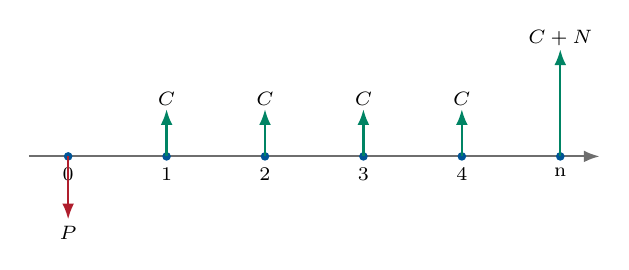
\begin{tikzpicture}[x=1.25cm, y=0.8cm]
  \draw[timeaxis] (-0.4,0) -- (5.4,0);
  \foreach \x/\l in {0/0, 1/1, 2/2, 3/3, 4/4, 5/n}
    { \node[timenode] at (\x,0) {}; \node[etiq, below=3pt] at (\x,0) {\l}; }
  \draw[fluxneg] (0,0) -- (0,-1.0);
  \node[etiq, below] at (0,-1.05) {$P$};
  \foreach \x in {1,2,3,4}
    { \draw[flux] (\x,0) -- (\x,0.75); \node[etiq, above] at (\x,0.75) {$C$}; }
  \draw[flux] (5,0) -- (5,1.7);
  \node[etiq, above] at (5,1.7) {$C+N$};
\end{tikzpicture}
\end{center}

\begin{exercice}[prix d'une obligation]
Une obligation de nominal $1\,000$~\euro{} porte un taux facial de $3{,}20\,\%$
et arrive à échéance dans $5$~ans. Le taux de marché est de $2{,}60\,\%$.
Calculer son prix et commenter sa position par rapport au pair.
\end{exercice}

\begin{corrige}
Le coupon annuel vaut $C = 32$~\euro. Avec $(1{,}026)^{-5} = 0{,}87956$ :
\[
  a_{\overline{5}|2{,}6\%} = \frac{1-0{,}87956}{0{,}026} = 4{,}63242,
  \qquad
  P = 32 \times 4{,}63242 + 1\,000 \times 0{,}87956 \approx 1\,027{,}79\ \text{\euro}.
\]
L'obligation cote au-dessus du pair, à $102{,}78\,\%$, parce que son taux facial
excède le taux de marché : elle sert un coupon plus généreux que ce que le
marché exige aujourd'hui, et cet avantage se paie.
\end{corrige}

\begin{exercice}[lecture inverse]
La même obligation se négocie à $985$~\euro. Déterminer son taux actuariel.
\end{exercice}

\begin{corrige}
On cherche $r$ tel que $32\,a_{\overline{5}|r} + 1\,000\,(1+r)^{-5} = 985$.
Deux essais encadrent la solution :
\[
  P(3{,}50\,\%) = 986{,}45\ \text{\euro},
  \qquad
  P(3{,}60\,\%) = 981{,}99\ \text{\euro}.
\]
Une interpolation linéaire donne
$r \approx 3{,}50 + 0{,}10 \times \tfrac{986{,}45-985}{986{,}45-981{,}99}
 \approx 3{,}53\,\%$.

C'est le taux de rendement interne de l'unité~2, appliqué à une obligation. On
l'appelle alors \emph{taux actuariel} ou \emph{rendement à l'échéance}.
\end{corrige}

\subsection{Généralisation : courbe des taux, coupon couru, sensibilité}

\begin{generalisation}{Trois compléments indispensables}
\textbf{La courbe des taux.} Il n'existe pas un taux, mais un taux par échéance.
Le taux \emph{zéro-coupon}\index{taux zéro-coupon} $z_k$ est celui qui actualise
un flux unique disponible en $k$. Le prix exact s'écrit alors
\[
  P \;=\; \sum_{k=1}^{n} \frac{C_k}{(1+z_k)^{k}} .
\]
Le taux actuariel $r$ n'est pas une donnée de marché : c'est le taux unique qui,
appliqué à tous les flux, reproduit ce prix. C'est un \emph{résumé} de la courbe,
pas un ingrédient du calcul.

\medskip
\textbf{Le coupon couru.} Entre deux détachements, le porteur acquiert
progressivement le droit au coupon suivant. Le \emph{coupon
couru}\index{coupon couru} est cette fraction acquise :
\[
  \mathrm{CC} \;=\; C \times \frac{\text{jours écoulés depuis le dernier détachement}}{\text{base}} .
\]
Les obligations se cotent \emph{pied de coupon}, c'est-à-dire hors coupon couru.
Le montant effectivement réglé est la somme des deux.

\medskip
\textbf{Duration et sensibilité.} La \emph{duration de
Macaulay}\index{duration} est la moyenne des dates de flux, pondérée par leurs
valeurs actuelles :
\[
  D \;=\; \frac{1}{P}\sum_{k=1}^{n} k \,\frac{C_k}{(1+r)^{k}} .
\]
Elle s'exprime en années et mesure la maturité \emph{économique} du titre. La
\emph{sensibilité}\index{sensibilité} $S = D/(1+r)$ en donne la lecture
opérationnelle : pour une variation $\Delta r$ du taux,
\[
  \frac{\Delta P}{P} \;\approx\; -\,S \times \Delta r .
\]
Cette relation est une approximation du premier ordre. La relation prix-taux
étant convexe, elle surestime toujours la baisse et sous-estime toujours la
hausse.
\end{generalisation}

\begin{center}
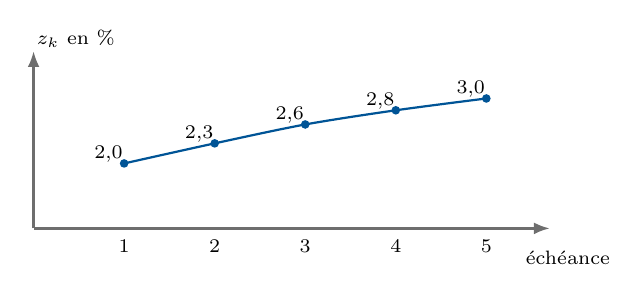
\begin{tikzpicture}[x=1.15cm, y=1.5cm]
  \draw[timeaxis] (0,0) -- (5.7,0);
  \draw[timeaxis] (0,0) -- (0,1.5);
  \node[etiq, right] at (5.4,-0.25) {échéance};
  \draw[thick, bleuactu] plot[smooth] coordinates
    {(1,0.55) (2,0.72) (3,0.88) (4,1.00) (5,1.10)};
  \foreach \x/\y/\l in {1/0.55/{2{,}0}, 2/0.72/{2{,}3}, 3/0.88/{2{,}6},
                        4/1.00/{2{,}8}, 5/1.10/{3{,}0}}
    { \node[timenode] at (\x,\y) {}; \node[etiq, above left=-1pt] at (\x,\y) {\l}; }
  \foreach \x in {1,2,3,4,5} { \node[etiq, below=3pt] at (\x,0) {\x}; }
  \node[etiq, above right] at (0,1.5) {$z_k$ en \%};
\end{tikzpicture}
\end{center}

\begin{exercice}[courbe non plate et coupon couru]
\textbf{(a)} Reprendre l'obligation précédente --- nominal $1\,000$~\euro, taux
facial $3{,}20\,\%$, maturité $5$~ans --- et la valoriser avec la courbe
zéro-coupon ci-dessus : $2{,}0\,\%$, $2{,}3\,\%$, $2{,}6\,\%$, $2{,}8\,\%$ et
$3{,}0\,\%$.

\medskip
\textbf{(b)} L'obligation cote $101{,}05\,\%$ pied de coupon. L'achat intervient
$73$~jours après le dernier détachement, en base exact/365. Déterminer le montant
réglé par l'acheteur.
\end{exercice}

\begin{corrige}
\textbf{(a)} Chaque flux est actualisé à \emph{son} taux :
\begin{center}\small
\begin{tabular}{ccrr}
\toprule
Année & Flux & $z_k$ & Flux actualisé \\
\midrule
1 & $32$    & $2{,}0\,\%$ & $31{,}37$ \\
2 & $32$    & $2{,}3\,\%$ & $30{,}58$ \\
3 & $32$    & $2{,}6\,\%$ & $29{,}63$ \\
4 & $32$    & $2{,}8\,\%$ & $28{,}65$ \\
5 & $1\,032$ & $3{,}0\,\%$ & $890{,}21$ \\
\midrule
\multicolumn{3}{r}{\textbf{Prix}} & $\mathbf{1\,010{,}44}$ \\
\bottomrule
\end{tabular}
\end{center}
Le prix tombe à $1\,010{,}44$~\euro, contre $1\,027{,}79$~\euro{} avec un taux
plat de $2{,}6\,\%$. La pente de la courbe pénalise les flux longs, et le
remboursement du nominal représente ici près de $88\,\%$ du prix.

\medskip
\textbf{(b)} Coupon couru : $\mathrm{CC} = 32 \times \tfrac{73}{365} = 6{,}40$~\euro.
\[
  \text{montant réglé} = 1\,010{,}50 + 6{,}40 = 1\,016{,}90\ \text{\euro}.
\]
La cotation pied de coupon existe pour que le prix affiché ne chute pas
artificiellement à chaque détachement : elle isole la variation de valeur
économique du simple écoulement du temps.
\end{corrige}

\begin{exercice}[choc de taux, approché puis exact]
Reprendre l'obligation valorisée à $1\,027{,}79$~\euro{} au taux plat de
$2{,}60\,\%$.

\textbf{(a)} Calculer sa duration de Macaulay et sa sensibilité.

\textbf{(b)} Estimer l'effet d'une hausse instantanée des taux de $100$~points de
base par la formule de sensibilité, puis recalculer le prix exact. Commenter
l'écart.
\end{exercice}

\begin{corrige}
\textbf{(a)} On pondère chaque date par la valeur actuelle de son flux :
\begin{center}\small
\begin{tabular}{crrr}
\toprule
$k$ & Flux & Valeur actuelle & $k \times$ VA \\
\midrule
1 & $32$    & $31{,}19$  & $31{,}19$ \\
2 & $32$    & $30{,}40$  & $60{,}80$ \\
3 & $32$    & $29{,}63$  & $88{,}89$ \\
4 & $32$    & $28{,}88$  & $115{,}51$ \\
5 & $1\,032$ & $907{,}70$ & $4\,538{,}50$ \\
\midrule
  & & $1\,027{,}79$ & $4\,834{,}89$ \\
\bottomrule
\end{tabular}
\end{center}
\[
  D = \frac{4\,834{,}89}{1\,027{,}79} = 4{,}704\ \text{ans},
  \qquad
  S = \frac{4{,}704}{1{,}026} = 4{,}585 .
\]
La duration est inférieure à la maturité de cinq ans, puisque les coupons
avancent le centre de gravité des flux.

\medskip
\textbf{(b)} Estimation par la sensibilité :
\[
  \frac{\Delta P}{P} \approx -4{,}585 \times 0{,}01 = -4{,}585\,\%
  \quad\Longrightarrow\quad
  \Delta P \approx -47{,}12\ \text{\euro},
  \quad P \approx 980{,}67\ \text{\euro}.
\]
Calcul exact à $3{,}60\,\%$ : $P = 981{,}99$~\euro, soit $\Delta P = -45{,}80$~\euro,
c'est-à-dire $-4{,}457\,\%$.

\medskip
L'approximation surestime la perte de $1{,}32$~\euro, soit près de $3\,\%$ de
l'effet estimé. C'est la \emph{convexité} : la courbe prix-taux étant convexe,
la tangente passe sous elle des deux côtés. Sur un portefeuille obligataire de
plusieurs milliards et pour un choc réglementaire pouvant dépasser $100$~points
de base, cet écart cesse d'être une subtilité.
\end{corrige}

\begin{pont}{Où cela sert dans Solvabilité~II}
Cette unité se retrouve dans un bilan prudentiel à trois endroits distincts.

\medskip
\emph{À l'actif.} Les placements obligataires sont inscrits en juste valeur.
Le prix calculé ici est celui qui figure au bilan.

\emph{Au passif.} La courbe zéro-coupon de cette unité a une version
réglementaire : la structure par terme des taux sans risque publiée par l'EIOPA.
C'est elle, et non un taux plat, qui actualise les flux de prestations dans la
meilleure estimation.

\emph{Dans le capital requis.} Le sous-module de risque de taux consiste à
déformer la courbe à la hausse puis à la baisse et à recalculer le bilan complet.
L'exercice~3.4 en est la version élémentaire, appliquée à un seul titre.

\medskip
Enfin, la duration est l'instrument qui permet de comparer un actif et un passif
sur la même échelle. Une compagnie dont les engagements ont une duration de
douze ans et les placements une duration de cinq ans subit une perte lorsque les
taux baissent, quand bien même chaque poste, pris isolément, se comporterait
normalement. Cette confrontation est l'objet de la gestion actif-passif, traitée
à l'unité~7.
\end{pont}

\begin{refreg}
\textbf{Références.} Directive 2009/138/CE, article~75 : les actifs sont
valorisés au montant pour lequel ils pourraient être échangés dans le cadre
d'une transaction conclue entre parties informées et consentantes. \\
Article~77, paragraphe~2 : actualisation des flux de trésorerie futurs au moyen
de la courbe des taux sans risque pertinente, publiée mensuellement par l'EIOPA
avec sa documentation technique. \\
Règlement délégué (UE) 2015/35 : sous-module de risque de taux d'intérêt.
\emph{[Références d'articles à préciser avant diffusion.]}
\end{refreg}

\subsection*{Notations introduites}
\begin{description}[leftmargin=3cm, style=nextline, font=\normalfont]
  \notation{N}{nominal de l'obligation}
  \notation{c,\ C = cN}{taux facial et coupon}
  \notation{P}{prix de l'obligation}
  \notation{z_k}{taux zéro-coupon d'échéance $k$}
  \notation{\mathrm{CC}}{coupon couru}
  \notation{D}{duration de Macaulay, en années}
  \notation{S = D/(1+r)}{sensibilité}
\end{description}

\newpage
\section{Un flux aléatoire}
\label{sec:U4}

Jusqu'ici, les flux étaient certains : seule leur date variait. On ajoute
maintenant l'ingrédient qui fait basculer du monde bancaire au monde de
l'assurance --- le flux peut ne pas avoir lieu.

C'est l'étage décisif de la progression. Une fois franchi, la phrase qui
gouverne tout le dispositif prudentiel devient lisible : \emph{un contrat
d'assurance est une variable aléatoire}, et le provisionner consiste à en
calculer l'espérance actualisée.

\subsection{La notion : espérance actualisée d'un flux conditionnel}

\begin{notion}{Deux ingrédients qui se multiplient}
Soit un flux $C$ payable en $n$ si un événement se réalise, et rien sinon.
Notons $p$ la probabilité de cet événement. La valeur actuelle probable est
\[
  V_0 \;=\; \frac{\mathbb{E}[C_n]}{(1+r)^n} \;=\; \frac{p \times C}{(1+r)^n} .
\]
La formule de l'unité~1 est intacte ; il s'y ajoute un unique facteur.

\medskip
Ce facteur est d'une autre nature que le taux, et cette distinction structure
tout le reste du cours. La probabilité $p$ relève d'une \emph{hypothèse
actuarielle} --- mortalité, fréquence de sinistre, comportement de l'assuré ---
estimée sur des données d'expérience. Le taux $r$ relève d'une \emph{donnée de
marché}. Les deux se multiplient, mais ne se justifient pas, ne se révisent pas
et ne se contrôlent pas de la même manière.
\end{notion}

\begin{center}
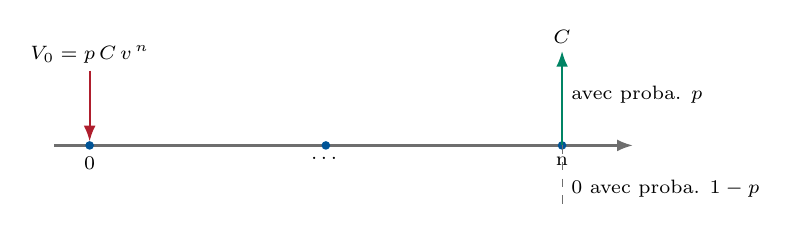
\begin{tikzpicture}[x=1.5cm, y=1cm]
  \draw[timeaxis] (-0.3,0) -- (4.6,0);
  \foreach \x/\l in {0/0, 2/{\dots}, 4/n}
    { \node[timenode] at (\x,0) {}; \node[etiq, below=3pt] at (\x,0) {\l}; }
  \draw[flux] (4,0) -- (4,1.2);
  \node[etiq, above] at (4,1.25) {$C$};
  \node[etiq, right] at (4.05,0.65) {avec proba. $p$};
  \draw[dashed, grisactu] (4,0) -- (4,-0.8);
  \node[etiq, right] at (4.05,-0.55) {$0$ avec proba. $1-p$};
  \draw[fluxneg] (0,0.95) -- (0,0.05);
  \node[etiq, above] at (0,1.0) {$V_0 = p\,C\,v^{\,n}$};
\end{tikzpicture}
\end{center}

\begin{exercice}[capital sous condition de survie]
Un contrat prévoit le versement d'un capital de $50\,000$~\euro{} dans $8$~ans,
à la condition que l'assuré, âgé de $52$~ans, soit alors en vie. La probabilité
de survie sur cet horizon est de $0{,}942$. Le taux d'actualisation est de
$2{,}40\,\%$.

Calculer la valeur actuelle probable de cet engagement, puis la comparer à celle
du même capital versé de façon certaine.
\end{exercice}

\begin{corrige}
Avec $(1{,}024)^{8} = 1{,}20893$ :
\[
  V_0 = \frac{0{,}942 \times 50\,000}{1{,}20893}
      = \frac{47\,100}{1{,}20893} \approx 38\,960\ \text{\euro}.
\]
Le même capital versé de façon certaine vaudrait
$50\,000/1{,}20893 \approx 41\,359$~\euro.

\medskip
L'écart, $2\,399$~\euro, représente exactement $5{,}8\,\%$ de la valeur certaine
--- c'est-à-dire la probabilité de décès sur la période. L'aléa se paie donc en
proportion stricte de sa probabilité, ce qui n'ira plus de soi à l'unité~5.
\end{corrige}

\begin{exercice}[lecture inverse]
Un engagement de même nature --- capital de $50\,000$~\euro{} à $8$~ans, taux de
$2{,}40\,\%$ --- est provisionné pour $38\,960$~\euro. Quelle probabilité de
survie cette provision suppose-t-elle ?
\end{exercice}

\begin{corrige}
On inverse la relation :
\[
  p = \frac{V_0 \times (1+r)^{n}}{C}
    = \frac{38\,960 \times 1{,}20893}{50\,000}
    = \frac{47\,100}{50\,000} = 0{,}942 .
\]
La provision suppose une probabilité de survie de $94{,}2\,\%$.

Cette lecture inverse est un réflexe de contrôle utile : à partir d'un montant
provisionné, on peut toujours reconstituer l'hypothèse implicite et juger si
elle est plausible.
\end{corrige}

\subsection{Généralisation : rentes viagères et flux croissants}

\begin{generalisation}{Une pondération par période, quelle qu'en soit l'origine}
\textbf{La table de mortalité.} Une table donne les effectifs $l_x$ d'un groupe
initial encore en vie à l'âge $x$. On en déduit la probabilité qu'une personne
d'âge $x$ soit encore en vie $k$ années plus tard :
\[
  {}_{k}p_x \;=\; \frac{l_{x+k}}{l_x},
  \qquad\text{et la probabilité de décéder l'année } k :\quad
  \frac{l_{x+k-1}-l_{x+k}}{l_x}.
\]

\medskip
\textbf{La rente viagère.} Une rente de $1$ versée en fin d'année tant que
l'assuré est en vie, sur $n$ années au plus, vaut
\[
  a_{x:\overline{n}|} \;=\; \sum_{k=1}^{n} {}_{k}p_x \; v^{\,k}.
\]
C'est la rente certaine de l'unité~2 dont chaque terme est pondéré par sa
probabilité de survenance.

\medskip
\textbf{Les flux croissants.} Si le flux, au lieu d'être aléatoire, croît au
taux constant $g$ à l'infini, la même somme admet une forme fermée --- le modèle
de Gordon-Shapiro\index{Gordon-Shapiro} :
\[
  V_0 \;=\; \sum_{k=1}^{\infty} \frac{D_1 (1+g)^{k-1}}{(1+r)^{k}}
       \;=\; \frac{D_1}{r-g},
  \qquad\text{sous réserve que } g < r .
\]

\medskip
\textbf{Ce qu'il faut retenir.} Dans les deux cas, on applique au facteur
d'actualisation $v^{\,k}$ un \emph{multiplicateur propre à chaque période} :
une probabilité de survie ici, un facteur de croissance là. La mécanique est
identique ; seule l'interprétation du multiplicateur change.
\end{generalisation}

\begin{exercice}[rente viagère temporaire]
Un assuré de $65$~ans perçoit une rente de $6\,000$~\euro{} en fin de chacune
des cinq prochaines années, tant qu'il est en vie. Le taux est de $2{,}00\,\%$.
La table de mortalité donne :
\begin{center}\small
\begin{tabular}{lrrrrrr}
\toprule
$x$   & $65$ & $66$ & $67$ & $68$ & $69$ & $70$ \\
$l_x$ & $100\,000$ & $98\,600$ & $97\,100$ & $95\,400$ & $93\,500$ & $91\,400$ \\
\bottomrule
\end{tabular}
\end{center}
Calculer la valeur actuelle probable de la rente, puis la comparer à celle d'une
rente certaine de même montant et de même durée.
\end{exercice}

\begin{corrige}
\begin{center}\small
\begin{tabular}{crrrr}
\toprule
$k$ & ${}_{k}p_{65}$ & $v^{\,k}$ & ${}_{k}p_{65}\,v^{\,k}$ & Flux actualisé \\
\midrule
1 & $0{,}98600$ & $0{,}98039$ & $0{,}96667$ & $5\,800{,}00$ \\
2 & $0{,}97100$ & $0{,}96117$ & $0{,}93329$ & $5\,599{,}77$ \\
3 & $0{,}95400$ & $0{,}94232$ & $0{,}89898$ & $5\,393{,}85$ \\
4 & $0{,}93500$ & $0{,}92385$ & $0{,}86380$ & $5\,182{,}77$ \\
5 & $0{,}91400$ & $0{,}90573$ & $0{,}82784$ & $4\,967{,}03$ \\
\midrule
  & & & $\mathbf{4{,}49057}$ & $\mathbf{26\,943{,}42}$ \\
\bottomrule
\end{tabular}
\end{center}
La rente viagère vaut environ $26\,943$~\euro, contre
$6\,000 \times a_{\overline{5}|2\%} = 6\,000 \times 4{,}71346 \approx 28\,281$~\euro{}
pour une rente certaine.

\medskip
L'écart de $1\,337$~\euro{} est le seul effet de la mortalité. Noter que le
coefficient $a_{65:\overline{5}|} = 4{,}4906$ se lit directement : la rente
« vaut » $4{,}49$~années de versement en valeur d'aujourd'hui, contre $4{,}71$
si elle était certaine.
\end{corrige}

\begin{exercice}[capital décès et flux croissant]
\textbf{(a)} Sur la même table et au même taux, un contrat verse un capital de
$100\,000$~\euro{} en fin de l'année du décès, si celui-ci survient dans les
cinq prochaines années. Calculer la valeur actuelle probable de cet engagement.

\medskip
\textbf{(b)} Une action versera un dividende de $4{,}20$~\euro{} l'an prochain,
puis croissant de $2{,}50\,\%$ par an indéfiniment. Le taux de rendement exigé
est de $7{,}00\,\%$. Évaluer l'action, puis mesurer l'effet d'une révision de la
croissance à $3{,}00\,\%$.
\end{exercice}

\begin{corrige}
\textbf{(a)} La probabilité de décéder l'année $k$ se lit sur les différences
d'effectifs :
\begin{center}\small
\begin{tabular}{crrr}
\toprule
$k$ & Proba. de décès & $v^{\,k}$ & Flux actualisé \\
\midrule
1 & $0{,}01400$ & $0{,}98039$ & $1\,372{,}55$ \\
2 & $0{,}01500$ & $0{,}96117$ & $1\,441{,}75$ \\
3 & $0{,}01700$ & $0{,}94232$ & $1\,601{,}95$ \\
4 & $0{,}01900$ & $0{,}92385$ & $1\,755{,}31$ \\
5 & $0{,}02100$ & $0{,}90573$ & $1\,902{,}03$ \\
\midrule
  & $0{,}08600$ & & $\mathbf{8\,073{,}59}$ \\
\bottomrule
\end{tabular}
\end{center}
L'engagement vaut environ $8\,074$~\euro. Contrôle de cohérence : la somme des
probabilités de décès, $0{,}086$, est bien le complément de la probabilité de
survie à cinq ans, $0{,}914$.

\medskip
\textbf{(b)} Au taux de croissance initial :
\[
  V_0 = \frac{4{,}20}{0{,}07-0{,}025} = \frac{4{,}20}{0{,}045} = 93{,}33\ \text{\euro}.
\]
Avec $g = 3{,}00\,\%$ : $V_0 = 4{,}20/0{,}04 = 105{,}00$~\euro.

\medskip
Une révision de $50$~points de base sur la croissance déplace la valeur de
$12{,}5\,\%$. Cette instabilité n'est pas un défaut du modèle : elle est la
propriété de tout engagement de très longue durée, et elle explique pourquoi la
sensibilité d'une meilleure estimation à ses hypothèses fait l'objet d'une
attention réglementaire particulière.
\end{corrige}

\begin{pont}{Où cela sert dans Solvabilité~II}
Cette unité est la définition même de la meilleure estimation. Le texte de la
directive énonce que celle-ci est la moyenne des flux de trésorerie futurs
\emph{pondérés par leur probabilité}, compte tenu de la valeur temporelle de
l'argent. Les deux ingrédients de la notion, et rien d'autre.

\medskip
Trois conséquences opérationnelles en découlent.

\emph{Les hypothèses doivent être réalistes.} Un best estimate se calcule avec
des probabilités d'expérience, sans marge de prudence. C'est une différence de
principe avec le provisionnement en normes françaises, qui recourt à des tables
réglementaires délibérément prudentes. Les deux bilans peuvent donc afficher des
provisions très différentes pour un même contrat, sans qu'aucun ne soit erroné.

\emph{L'écart de provision a désormais deux sources.} L'unité~2 en avait
identifié une, l'actualisation. Celle-ci en apporte la seconde, le choix des
hypothèses. Ensemble, elles expliquent l'essentiel de la divergence entre bilan
comptable et bilan prudentiel.

\emph{La sensibilité aux hypothèses devient un objet en soi.} L'exercice~4.4
montre qu'un déplacement minime d'une hypothèse de long terme produit un effet
majeur sur la valeur.

\medskip
Il manque encore un ingrédient, et c'est celui qui rendra l'aléa non
proportionnel à sa probabilité : le contrat peut donner à l'assuré un
\emph{choix}. C'est l'objet de l'unité~5.
\end{pont}

\begin{refreg}
\textbf{Références.} Directive 2009/138/CE, article~77, paragraphe~2 : la
meilleure estimation correspond à la moyenne pondérée par leur probabilité des
flux de trésorerie futurs, compte tenu de la valeur temporelle de l'argent. \\
Le même article prévoit que le calcul repose sur des informations actualisées et
crédibles et sur des hypothèses réalistes. \\
Règlement délégué (UE) 2015/35 : hypothèses relatives aux options et garanties
contractuelles, et segmentation. \emph{[Références d'articles à préciser avant
diffusion.]}
\end{refreg}

\subsection*{Notations introduites}
\begin{description}[leftmargin=2.4cm, style=nextline, font=\normalfont]
  \notation{p}{probabilité de réalisation d'un flux}
  \notation{l_x}{effectif survivant à l'âge $x$ dans la table}
  \notation{{}_{k}p_x}{probabilité qu'une tête d'âge $x$ survive $k$ ans}
  \notation{a_{x:\overline{n}|}}{valeur actuelle d'une rente viagère temporaire de 1 versée pour $n$ années à une personne âgée de $x$ ans.}
  \notation{D_1}{premier dividende attendu}
  \notation{g}{taux de croissance des flux}
\end{description}

\newpage
\section{Un flux optionnel}
\label{sec:U5}

L'unité~4 a montré qu'un flux aléatoire se valorise en pondérant chaque issue par
sa probabilité. On ajoute ici le dernier ingrédient avant le contrat d'assurance
complet : le montant versé ne dépend plus seulement du hasard, mais d'un
\emph{choix} exercé au vu de ce hasard.

Ce déplacement est plus profond qu'il n'y paraît. Il invalide la méthode
précédente : espérer les issues sous leur probabilité réelle donnera désormais
un résultat faux. La raison de cet échec, et sa réparation, sont l'objet de
cette unité --- et le prérequis direct des modèles stochastiques de l'unité~8.

\subsection{La notion : payoff et asymétrie}

\begin{notion}{Un flux qui ne peut pas être négatif}
Une option d’achat (\emph{call}\index{call}) au prix d'exercice $K$ donne le droit d'acheter un \textit{sous-jacent} à ce prix $K$. Toutefois cet achat n’est pas obligatoire : le détenteur de l’option ne l’exerce que si cela lui profite. Le flux terminal, ou \emph{payoff}, vaut donc
\[
  C_T \;=\; \max(S_T - K,\; 0),
\]
et symétriquement pour une option de vente (\emph{put}\index{put}), droit de vendre, avec un flux terminal :
$P_T = \max(K - S_T,\; 0)$.

\medskip
L'opérateur $\max(\cdot,0)$ est tout ce qui distingue cette unité des
précédentes, et il change tout. La relation entre le sous-jacent et le flux
cesse d'être linéaire : les issues défavorables sont tronquées, les favorables
conservées. C'est l'\emph{asymétrie}\index{asymétrie}, et c'est très exactement
la forme d'une garantie d'assurance.
\end{notion}

\begin{center}
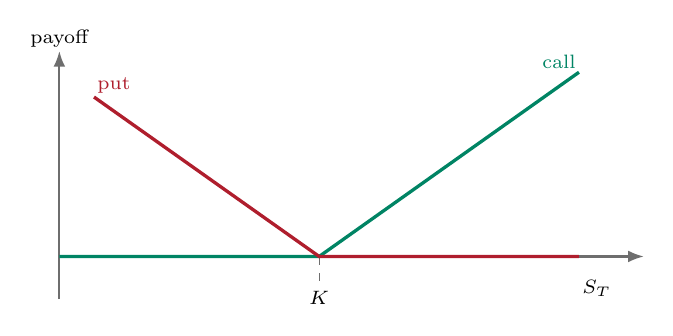
\begin{tikzpicture}[x=0.055cm, y=0.045cm]
  \draw[timeaxis] (0,0) -- (135,0);
  \draw[timeaxis] (0,-12) -- (0,58);
  \node[etiq, right] at (120,-9) {$S_T$};
  \node[etiq, above] at (0,58) {payoff};
  \draw[dashed, grisactu] (60,0) -- (60,-9);
  \node[etiq, below] at (60,-9) {$K$};
  \draw[very thick, vertactu] (0,0) -- (60,0) -- (120,52);
  \node[etiq, above left, vertactu] at (120,52) {call};
  \draw[very thick, rougeactu] (8,45) -- (60,0) -- (120,0);
  \node[etiq, above right, rougeactu] at (8,45) {put};
\end{tikzpicture}
\end{center}

\begin{exercice}[lecture d'un payoff]
Un call de prix d'exercice $K = 100$ est acheté $7{,}50$~\euro. Établir le payoff
puis le résultat net pour l'acheteur si le sous-jacent vaut à l'échéance
$88$, $100$, $104$ ou $121$. Déterminer le point mort.
\end{exercice}

\begin{corrige}
\begin{center}\small
\begin{tabular}{rrrr}
\toprule
$S_T$ & Payoff & Prime & Résultat net \\
\midrule
$88$  & $0$  & $-7{,}50$ & $-7{,}50$ \\
$100$ & $0$  & $-7{,}50$ & $-7{,}50$ \\
$104$ & $4$  & $-7{,}50$ & $-3{,}50$ \\
$121$ & $21$ & $-7{,}50$ & $+13{,}50$ \\
\bottomrule
\end{tabular}
\end{center}
Le point mort s'établit à $S_T = K + 7{,}50 = 107{,}50$.

\medskip
La perte est plafonnée à la prime, le gain ne l'est pas. Une compagnie qui
\emph{vend} une garantie occupe la position exactement inverse : gain plafonné à
la prime encaissée, perte non bornée. C'est la structure économique de tout
contrat d'assurance.
\end{corrige}

\begin{exercice}[pourquoi l'espérance réelle échoue]
Un actif vaut $100$ aujourd'hui. Dans un an, il vaudra $120$ avec une probabilité
de $60\,\%$, ou $90$ avec une probabilité de $40\,\%$. Le taux sans risque est de
$3\,\%$.

\textbf{(a)} Calculer l'espérance actualisée du sous-jacent selon la méthode de
l'unité~4. Comparer au prix observé, $100$. Que constate-t-on ?

\textbf{(b)} Un call de prix d'exercice $K=100$ est écrit sur cet actif. Calculer
son espérance actualisée par la même méthode.
\end{exercice}

\begin{corrige}
\textbf{(a)} $\mathbb{E}[S_1] = 0{,}6 \times 120 + 0{,}4 \times 90 = 108$, d'où
\[
  \frac{108}{1{,}03} = 104{,}85 \;\neq\; 100 .
\]
La méthode de l'unité~4 ne reproduit pas le prix de marché. L'écart n'est pas une erreur : il rémunère le risque supporté par le détenteur de l'actif. Un actif risqué ne s'actualise pas au taux sans risque.

\medskip
\textbf{(b)} Payoffs : $\max(120-100,0) = 20$ et $\max(90-100,0) = 0$.
\[
  \frac{0{,}6 \times 20 + 0{,}4 \times 0}{1{,}03} = \frac{12}{1{,}03} = 11{,}65 .
\]
Ce résultat est \emph{faux}, et pour la même raison qu'en (a) : il actualise un
flux risqué au taux sans risque. Mais il est ici impossible de le corriger par
une prime de risque ad hoc --- le risque d'une option n'est pas celui de son
sous-jacent, et il change à chaque instant. Il faut une autre méthode.
\end{corrige}

\subsection{Généralisation : réplication et repondération}

\begin{generalisation}{Ne pas prévoir, mais reproduire}
\textbf{L'idée.} Plutôt que de prédire la valeur de l'option, on construit un
portefeuille qui verse \emph{exactement} les mêmes flux dans tous les états de la nature.
Par absence d'opportunité d'arbitrage --- principe posé à l'unité~2 --- l'option
et ce portefeuille ont nécessairement le même prix.

\medskip
\textbf{Le modèle à une période.} Le sous-jacent vaut $S_0$ et prendra la valeur
$S_u = u\,S_0$ ou $S_d = d\,S_0$, avec $d < 1+r < u$. On cherche un portefeuille
composé de $\Delta$ unités de sous-jacent et de $B$ placé au taux sans risque,
qui reproduise les flux terminaux $(C_u, C_d)$. Ce portefeuille doit donc être tel que :\\
\begin{description}[leftmargin=3cm, style=nextline, font=\normalfont]
  \notation{\text{(cas de hausse)}}{$\Pi_u = \Delta S_u + B(1+r) = C_u$}
  \notation{\text{(cas de baisse)}}{$\Pi_d = \Delta S_d + B(1+r) = C_d$}
\end{description}

En résolvant, on trouve :\\

\[
  \Delta \;=\; \frac{C_u - C_d}{S_u - S_d},
  \qquad
  B \;=\; \frac{C_u - \Delta\,S_u}{1+r},
\]

L’hypothèse d’absence d'opportunité d'arbitrage – principe posé à l'unité 2 — conduit à la conclure que l'option et ce portefeuille ont nécessairement le même prix :\\
\[
  C_0 \;=\; \Delta\,S_0 + B .
\]


\medskip
\textbf{La repondération.} En réorganisant ces trois relations, le prix se
réécrit sous une forme remarquable :
\[
  C_0 \;=\; \frac{q\,C_u + (1-q)\,C_d}{1+r},
  \qquad\text{avec}\qquad
  q \;=\; \frac{(1+r) - d}{u - d}.
\]
Le prix est donc une espérance actualisée, comme à l'unité~4 --- mais calculée
avec $q$ au lieu de la probabilité réelle $p$.

\medskip
\textbf{Ce qu'est $q$, et ce qu'il n'est pas.} La quantité $q$, dite
\emph{probabilité risque-neutre}\index{probabilité risque-neutre}, est comprise
entre $0$ et $1$ et se manipule comme une probabilité. Mais elle ne décrit
\emph{aucune} croyance sur l'avenir : elle ne dépend pas de $p$, et $p$
n'apparaît nulle part dans le prix. C'est un artefact de calcul, la pondération
qui rend l'actualisation au taux sans risque légitime.

\medskip
\textbf{L'extension.} Sur plusieurs périodes, on répète l'opération de proche en
proche, en partant des dates terminales et en remontant. Lorsque le nombre de
périodes devient très grand, cette récurrence converge vers une intégrale : c'est
la formule de Black-Scholes. Lorsque les branches deviennent trop nombreuses pour
être énumérées, on tire au sort des trajectoires sous $q$ et l'on moyenne : c'est
la \emph{simulation de Monte-Carlo}\index{Monte-Carlo}.
\end{generalisation}

\begin{center}
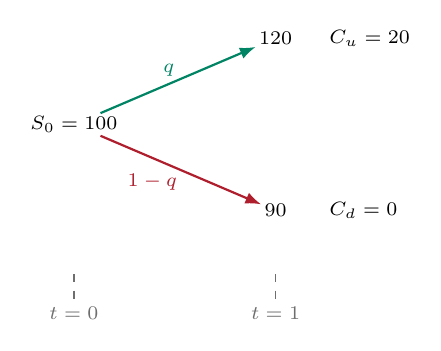
\begin{tikzpicture}[x=1.6cm, y=0.95cm]
  \node[etiq] (a) at (0,0) {$S_0 = 100$};
  \node[etiq] (u) at (1.6,1.15) {$120$};
  \node[etiq] (d) at (1.6,-1.15) {$90$};
  \draw[flux] (a) -- (u) node[midway, above left, etiq] {$q$};
  \draw[fluxneg] (a) -- (d) node[midway, below left, etiq] {$1-q$};
  \node[etiq, right] at (2.0,1.15) {$C_u = 20$};
  \node[etiq, right] at (2.0,-1.15) {$C_d = 0$};
  \draw[dashed, grisactu] (0,-2.0) -- (0,-2.4) node[below, etiq] {$t=0$};
  \draw[dashed, grisactu] (1.6,-2.0) -- (1.6,-2.4) node[below, etiq] {$t=1$};
\end{tikzpicture}
\end{center}

\begin{exercice}[réplication et repondération]
Reprendre les données de l'exercice~5.2 : $S_0 = 100$, $u = 1{,}20$,
$d = 0{,}90$, $r = 3\,\%$, call de prix d'exercice $K = 100$.

\textbf{(a)} Construire le portefeuille de réplication et en déduire le prix.

\textbf{(b)} Calculer $q$ et retrouver le prix par la formule de repondération.

\textbf{(c)} Que devient le prix si la probabilité réelle de hausse passe de
$60\,\%$ à $80\,\%$ ?
\end{exercice}

\begin{corrige}
\textbf{(a)} Payoffs : $C_u = 20$, $C_d = 0$.
\[
  \Delta = \frac{20-0}{120-90} = 0{,}6667,
  \qquad
  B = \frac{20 - 0{,}6667 \times 120}{1{,}03} = \frac{-60}{1{,}03} = -58{,}25 .
\]
\[
  C_0 = 0{,}6667 \times 100 - 58{,}25 = 8{,}41 .
\]
Le portefeuille consiste à détenir deux tiers d'unité de sous-jacent, financés
pour $58{,}25$ par emprunt. Vérification dans l'issue basse :
$0{,}6667 \times 90 - 58{,}25 \times 1{,}03 = 60 - 60 = 0 = C_d$.

\medskip
\textbf{(b)} $q = \dfrac{1{,}03 - 0{,}90}{1{,}20-0{,}90} = \dfrac{0{,}13}{0{,}30} = 0{,}4333$.
\[
  C_0 = \frac{0{,}4333 \times 20 + 0{,}5667 \times 0}{1{,}03} = \frac{8{,}6667}{1{,}03} = 8{,}41 .
\]
Les deux méthodes coïncident, comme elles le doivent.

\medskip
\textbf{(c)} Le prix ne change pas : il reste $8{,}41$. La probabilité réelle
n'entre dans aucune des deux formules.

\medskip
Ce résultat déconcerte, et c'est normal. Il signifie qu'anticiper une hausse ne
rend pas l'option plus chère : ce qui la valorise n'est pas l'espérance de gain,
mais le coût de sa reproduction. Noter au passage l'écart avec le calcul erroné
de l'exercice~5.2 : $8{,}41$ contre $11{,}65$, soit une surestimation de $38{,}5\,\%$.
\end{corrige}

\begin{exercice}[garantie plancher sur un contrat d'épargne]
Un contrat d'épargne investit $10\,000$~\euro{} sur un support dont la valeur
peut, chaque année, progresser de $15\,\%$ ou reculer de $10\,\%$. Le taux sans
risque est de $2\,\%$. Le contrat garantit à l'assuré de récupérer au minimum sa
mise au terme de deux ans.

\textbf{(a)} Construire l'arbre des valeurs du support sur deux périodes.

\textbf{(b)} Valoriser la garantie, c'est-à-dire l'engagement de l'assureur de
combler l'écart si la valeur finale est inférieure à $10\,000$~\euro.

\textbf{(c)} Commenter ce que représente ce montant pour l'assureur.
\end{exercice}

\begin{corrige}
\textbf{(a)} Avec $u = 1{,}15$ et $d = 0{,}90$ :
\begin{center}\small
\begin{tabular}{lrr}
\toprule
Trajectoire & Valeur en $t=2$ & Coût de la garantie \\
\midrule
$uu$ & $13\,225$ & $0$ \\
$ud$ et $du$ & $10\,350$ & $0$ \\
$dd$ & $8\,100$ & $1\,900$ \\
\bottomrule
\end{tabular}
\end{center}

\medskip
\textbf{(b)} $q = \dfrac{1{,}02-0{,}90}{1{,}15-0{,}90} = \dfrac{0{,}12}{0{,}25} = 0{,}48$.

La garantie ne se déclenche que sur la trajectoire $dd$, de probabilité
risque-neutre $(1-q)^2 = 0{,}52^2 = 0{,}2704$ :
\[
  V_0 = \frac{0{,}2704 \times 1\,900}{(1{,}02)^{2}}
      = \frac{513{,}76}{1{,}0404} \approx 493{,}81\ \text{\euro}.
\]

\medskip
\textbf{(c)} Ce montant, soit $4{,}94\,\%$ de la mise, est ce que coûterait à
l'assureur la couverture de sa promesse sur le marché. Il ne s'agit pas d'une
perte probable, mais du prix d'un engagement.

C'est très exactement la nature de la \emph{valeur temps des options et
garanties} incluse dans une meilleure estimation : un contrat d'épargne à
garantie plancher vaut davantage que la seule projection de son support, et
l'écart est une option que l'assureur a vendue sans toujours l'avoir facturée.
\end{corrige}

\begin{pont}{Où cela sert dans Solvabilité~II}
Les contrats d'assurance sont truffés d'options, le plus souvent implicites et
détenues par l'assuré : garantie de taux minimum, participation aux bénéfices,
faculté de rachat, option de conversion en rente. Toutes ont la forme
asymétrique de cette unité, et toutes sont exercées au moment le moins favorable
à l'assureur.

\medskip
Trois conséquences directes.

\emph{La meilleure estimation ne peut pas ignorer ces options.} La directive
impose de tenir compte de la valeur des garanties financières et des options
contractuelles. Une projection en scénario central les manquerait par
construction : dans un scénario moyen, une garantie plancher ne se déclenche
jamais.

\emph{C'est pourquoi les modèles vie sont stochastiques.} Là où un portefeuille
non-vie se projette sur une cadence déterministe, un portefeuille épargne exige
de simuler des milliers de trajectoires --- sous la probabilité $q$ de cette
unité --- et de moyenner. L'unité~8 en fait la mise en \oe uvre.

\emph{Les hypothèses comportementales redeviennent réelles.} Le taux de rachat
des assurés, lui, n'est pas une probabilité risque-neutre : c'est une hypothèse
d'expérience au sens de l'unité~4. Un modèle vie fait donc coexister les deux
natures de probabilité, et les confondre est l'une des erreurs les plus
fréquentes.
\end{pont}

\begin{refreg}
\textbf{Références.} Directive 2009/138/CE, article~77, paragraphe~2 : le calcul
de la meilleure estimation tient compte de la valeur des garanties financières et
de toute option contractuelle incluse dans les contrats. \\
Article~79 : évaluation des garanties financières et des options contractuelles,
et exigence que les hypothèses relatives à leur exercice soient réalistes et
fondées sur des informations actuelles et crédibles. \\
Règlement délégué (UE) 2015/35 : méthodes de valorisation et cohérence avec les
données de marché observables. \emph{[Références d'articles à préciser avant
diffusion.]}
\end{refreg}

\subsection*{Notations introduites}
\begin{description}[leftmargin=2.4cm, style=nextline, font=\normalfont]
  \notation{K}{prix d'exercice}
  \notation{S_T}{valeur du sous-jacent à l'échéance}
  \notation{u,\ d}{facteurs de hausse et de baisse}
  \notation{\Delta}{quantité de sous-jacent du portefeuille de réplication}
  \notation{B}{montant placé au taux sans risque}
  \notation{q}{probabilité risque-neutre}
\end{description}

\newpage
\section{Un contrat d'assurance}
\label{sec:U6}

Les cinq unités précédentes ont introduit, une par une, toutes les pièces
nécessaires : l'actualisation, les dates multiples, la dépendance aux taux de
marché, l'aléa, l'optionalité. Il n'y a rien de neuf à apprendre ici. On les
assemble.

Le résultat porte un nom réglementaire --- la meilleure estimation --- mais il
n'est rien d'autre que la valeur actuelle probable d'un échéancier. Cette unité
est l'atterrissage de toute la progression.

\subsection{La notion : l'échéancier probabilisé d'un contrat}

\begin{notion}{Un contrat est une variable aléatoire}
Un contrat d'assurance engage l'assureur à verser des prestations dont le
montant et la date sont incertains. Il est donc décrit par une suite de flux
\emph{attendus} $(\mathbb{E}[F_1],\dots,\mathbb{E}[F_n])$, et sa valeur est
\[
  \mathrm{BE} \;=\; \sum_{k=1}^{n} \frac{\mathbb{E}[F_k]}{(1+z_k)^{k}} .
\]
Chaque ingrédient a été vu séparément : l'espérance vient de l'unité~4, les
dates multiples de l'unité~2, les taux $z_k$ lus sur la courbe de l'unité~3.

\medskip
En assurance non-vie, les flux attendus se déduisent d'une \emph{cadence de
règlement}\index{cadence de règlement} : la charge ultime $S$ d'un exercice de
survenance se règle progressivement selon un profil $c_1,\dots,c_n$ observé sur
l'historique, avec $\sum_k c_k = 1$. Alors $\mathbb{E}[F_k] = S \times c_k$.
\end{notion}

\begin{center}
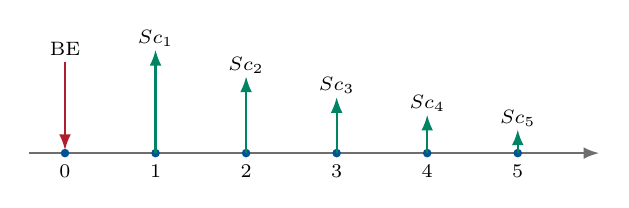
\begin{tikzpicture}[x=1.15cm, y=0.75cm]
  \draw[timeaxis] (-0.4,0) -- (5.9,0);
  \foreach \x/\l in {0/0, 1/1, 2/2, 3/3, 4/4, 5/5}
    { \node[timenode] at (\x,0) {}; \node[etiq, below=3pt] at (\x,0) {\l}; }
  \draw[flux] (1,0) -- (1,1.75); \node[etiq, above] at (1,1.75) {$Sc_1$};
  \draw[flux] (2,0) -- (2,1.30); \node[etiq, above] at (2,1.30) {$Sc_2$};
  \draw[flux] (3,0) -- (3,0.95); \node[etiq, above] at (3,0.95) {$Sc_3$};
  \draw[flux] (4,0) -- (4,0.65); \node[etiq, above] at (4,0.65) {$Sc_4$};
  \draw[flux] (5,0) -- (5,0.40); \node[etiq, above] at (5,0.40) {$Sc_5$};
  \draw[fluxneg] (0,1.55) -- (0,0.05);
  \node[etiq, above] at (0,1.6) {$\mathrm{BE}$};
\end{tikzpicture}
\end{center}

\begin{exercice}[meilleure estimation en non-vie]
Un portefeuille de responsabilité civile automobile présente une charge ultime
estimée à $8\,000\,000$~\euro{} au titre des sinistres déjà survenus. La cadence
de règlement observée est de $40\,\%$, $25\,\%$, $18\,\%$, $12\,\%$ et $5\,\%$,
les règlements intervenant en fin d'année. Le taux d'actualisation est de
$2{,}20\,\%$, constant.

Calculer la meilleure estimation de la provision pour sinistres à payer, puis la
comparer à la provision non actualisée.
\end{exercice}

\begin{corrige}
\begin{center}\small
\begin{tabular}{crrrr}
\toprule
Année & Part réglée & Flux attendu & Facteur & Flux actualisé \\
\midrule
1 & $40\,\%$ & $3\,200\,000$ & $0{,}97847$ & $3\,131\,115$ \\
2 & $25\,\%$ & $2\,000\,000$ & $0{,}95741$ & $1\,914\,821$ \\
3 & $18\,\%$ & $1\,440\,000$ & $0{,}93680$ & $1\,348\,993$ \\
4 & $12\,\%$ & $960\,000$    & $0{,}91663$ & $879\,970$ \\
5 & $5\,\%$  & $400\,000$    & $0{,}89690$ & $358\,761$ \\
\midrule
\multicolumn{3}{r}{\textbf{Meilleure estimation}} & & $\mathbf{7\,633\,661}$ \\
\bottomrule
\end{tabular}
\end{center}
La provision non actualisée s'élève à $8\,000\,000$~\euro. L'écart, soit
$366\,339$~\euro{} ou $4{,}58\,\%$, est le seul effet de l'actualisation.

\medskip
Cet écart dépend de deux choses : le niveau des taux, et la longueur de la
cadence. Sur une branche à déroulement long --- la responsabilité civile
médicale, la construction --- où les règlements s'étalent sur quinze ou vingt
ans, il peut dépasser $15\,\%$.
\end{corrige}

\begin{exercice}[l'écart avec la provision comptable]
Le même portefeuille est provisionné en normes françaises à $8\,600\,000$~\euro,
la réglementation imposant une évaluation prudente et sans actualisation.

Décomposer l'écart entre cette provision et la meilleure estimation calculée
ci-dessus, en distinguant ses deux sources.
\end{exercice}

\begin{corrige}
\[
  8\,600\,000 - 7\,633\,661 = 966\,339\ \text{\euro}.
\]
Cet écart se décompose exactement en deux termes :
\begin{center}\small
\begin{tabular}{lrl}
\toprule
Source & Montant & Origine \\
\midrule
Marge de prudence   & $600\,000$ & hypothèses prudentes contre réalistes \\
Actualisation       & $366\,339$ & valeur temporelle de l'argent \\
\midrule
\textbf{Écart total} & $\mathbf{966\,339}$ & \\
\bottomrule
\end{tabular}
\end{center}

\medskip
Les deux sources sont de nature différente et se justifient devant un contrôleur
par des arguments distincts. La marge de prudence relève du choix des hypothèses,
étudié à l'unité~4 ; l'actualisation relève de la mécanique financière, étudiée
à l'unité~2.

Le passage à la meilleure estimation \emph{libère} donc des fonds propres --- ici
près d'un million d'euros. C'est l'un des effets les plus visibles du passage
en normes prudentielles, et l'une des questions les plus fréquentes en contrôle.
\end{corrige}

\subsection{Généralisation : frontière des contrats et marge de risque}

\begin{generalisation}{Ce que l'on projette, et ce que l'on ajoute}
\textbf{La frontière des contrats.} Tous les flux futurs ne sont pas à
provisionner. La \emph{frontière du contrat}\index{frontière des contrats}
délimite les engagements que l'assureur ne peut plus refuser : les primes
futures ne sont incluses que s'il ne dispose ni du droit de résilier, ni de
celui de refuser la prime, ni de celui d'en modifier librement le niveau. Un
contrat annuel tacitement reconductible, résiliable à l'échéance, a donc une
frontière d'un an --- même si le client restera vraisemblablement dix ans.

C'est une frontière \emph{juridique}, pas comportementale. Elle produit des
résultats contre-intuitifs, et elle est la source d'erreur la plus fréquente
dans un calcul de meilleure estimation vie.

\medskip
\textbf{La meilleure estimation est nette.} On projette tous les flux liés au
contrat : prestations, frais de gestion et d'acquisition, et primes à recevoir
en signe opposé.
\[
  \mathrm{BE} \;=\; \sum_{k} \frac{\mathbb{E}[\text{prestations}_k] + \mathbb{E}[\text{frais}_k]
    - \mathbb{E}[\text{primes}_k]}{(1+z_k)^{k}} .
\]
Une meilleure estimation peut donc être négative, ce qu'aucune provision
comptable ne permet.

\medskip
\textbf{La marge de risque.} La meilleure estimation est une espérance : par
construction, elle sera insuffisante une fois sur deux. Les provisions
techniques y ajoutent une \emph{marge de risque}\index{marge de risque},
définie comme le coût d'immobilisation du capital qu'un repreneur exigerait
pour porter les engagements jusqu'à leur extinction :
\[
  \mathrm{MR} \;=\; \mathrm{CoC} \times \sum_{k \geq 0}
    \frac{\mathrm{SCR}_k}{(1+z_{k+1})^{k+1}},
  \qquad \mathrm{CoC} = 6\,\% .
\]
On retrouve, une fois encore, une somme de flux actualisés --- les $\mathrm{SCR}_k$
étant les capitaux requis projetés année après année.

\medskip
\[
  \boxed{\ \text{Provisions techniques} \;=\; \mathrm{BE} \;+\; \mathrm{MR}\ }
\]
\end{generalisation}

\begin{exercice}[frontière des contrats]
Pour chacune des situations suivantes, indiquer si les primes futures entrent
dans la meilleure estimation, et justifier.

\textbf{(a)} Un contrat automobile annuel, tacitement reconductible, que
l'assureur peut résilier à chaque échéance.

\textbf{(b)} Un contrat d'épargne à versements libres, sans engagement de
l'assuré ni faculté de refus par l'assureur.

\textbf{(c)} Un contrat de prévoyance décès à prime nivelée sur vingt ans, que
l'assureur ne peut ni résilier ni retarifer.
\end{exercice}

\begin{corrige}
\textbf{(a)} \emph{Non.} La faculté de résiliation annuelle place la frontière à
l'échéance suivante. Le fait que le contrat sera vraisemblablement reconduit dix
ans est sans effet : le critère est juridique, non comportemental.

\medskip
\textbf{(b)} \emph{Non} pour les versements futurs, qui ne sont pas des
engagements : l'assuré est libre de ne pas verser. En revanche, l'épargne déjà
constituée est intégralement provisionnée, avec toutes les garanties qui s'y
attachent.

\medskip
\textbf{(c)} \emph{Oui}, sur vingt ans. L'assureur est engagé pour toute la
durée sans pouvoir modifier le tarif : les primes futures sont dans la frontière
et viennent en déduction de la meilleure estimation.

\medskip
Le cas (c) illustre la possibilité d'une meilleure estimation négative : si la
valeur actuelle des primes excède celle des prestations et des frais, le contrat
constitue un actif, non un passif. C'est économiquement juste et comptablement
impossible en normes françaises.
\end{corrige}

\begin{exercice}[provisions techniques complètes]
Reprendre le portefeuille de l'exercice~6.1, dont la meilleure estimation
s'établit à $7\,633\,661$~\euro. Le capital de solvabilité requis au titre de ce
portefeuille est projeté comme suit, en fin de chaque année :
\begin{center}\small
\begin{tabular}{lrrrrr}
\toprule
Année $k$ & $0$ & $1$ & $2$ & $3$ & $4$ \\
$\mathrm{SCR}_k$ & $1\,200\,000$ & $780\,000$ & $460\,000$ & $220\,000$ & $80\,000$ \\
\bottomrule
\end{tabular}
\end{center}
Le taux d'actualisation reste de $2{,}20\,\%$ et le coût du capital de $6\,\%$.

Calculer la marge de risque, puis les provisions techniques.
\end{exercice}

\begin{corrige}
Chaque $\mathrm{SCR}_k$ est actualisé sur $k+1$ périodes :
\begin{center}\small
\begin{tabular}{crrr}
\toprule
$k$ & $\mathrm{SCR}_k$ & Facteur $(1{,}022)^{-(k+1)}$ & Montant actualisé \\
\midrule
0 & $1\,200\,000$ & $0{,}97847$ & $1\,174\,168$ \\
1 & $780\,000$    & $0{,}95741$ & $746\,780$ \\
2 & $460\,000$    & $0{,}93680$ & $430\,928$ \\
3 & $220\,000$    & $0{,}91663$ & $201\,660$ \\
4 & $80\,000$     & $0{,}89690$ & $71\,752$ \\
\midrule
\multicolumn{3}{r}{\textbf{Somme}} & $\mathbf{2\,625\,289}$ \\
\bottomrule
\end{tabular}
\end{center}
\[
  \mathrm{MR} = 6\,\% \times 2\,625\,289 = 157\,517\ \text{\euro}.
\]
\[
  \text{Provisions techniques} = 7\,633\,661 + 157\,517 = 7\,791\,178\ \text{\euro}.
\]

\medskip
La marge de risque représente ici $2{,}06\,\%$ de la meilleure estimation. Sur
une branche à déroulement long, où les $\mathrm{SCR}$ projetés restent élevés
pendant quinze ans, cette proportion est sensiblement plus forte.

Noter que même après ajout de la marge de risque, les provisions techniques
restent inférieures de $808\,822$~\euro{} à la provision comptable de
$8\,600\,000$~\euro.
\end{corrige}

\begin{pont}{Où cela sert dans Solvabilité~II}
Cette unité \emph{est} le passif du bilan prudentiel. Rien de plus n'est requis
pour le construire, du moins en assurance non-vie.

\medskip
La progression complète se relit d'un trait. Un flux certain, actualisé
(unité~1). Plusieurs dates, donc une somme (unité~2). Des taux lus sur la courbe
EIOPA plutôt qu'un taux plat (unité~3). Des flux pondérés par leur probabilité
d'occurrence (unité~4). Une pondération risque-neutre lorsque le contrat comporte
des options (unité~5). Enfin l'assemblage, augmenté de la marge de risque
(unité~6). Chaque étage n'ajoutait qu'un ingrédient, et le dernier ne fait que
les réunir.

\medskip
Deux prolongements restent à construire, et ils forment la suite du cours.

\emph{L'actif face au passif.} Une meilleure estimation ne se calcule pas
isolément : sa valeur dépend du rendement des placements qui la couvrent, et
réciproquement les décisions d'investissement dépendent du profil des
engagements. Cette interaction est l'objet de la gestion actif-passif, à
l'unité~7.

\emph{La projection stochastique.} En assurance vie, les options de l'unité~5
--- garanties de taux, participation aux bénéfices, rachats --- interdisent la
projection déterministe employée ici. Il faut simuler des milliers de
trajectoires et moyenner : c'est l'unité~8.

\medskip
La méthode reste pourtant la même dans les deux cas : une espérance de flux
actualisés. Seule la manière de calculer l'espérance change.
\end{pont}

\begin{refreg}
\textbf{Références.} Directive 2009/138/CE, article~76 : les provisions
techniques correspondent au montant que les entreprises devraient payer pour
transférer immédiatement leurs engagements à une autre entreprise. \\
Article~77 : la valeur des provisions techniques est égale à la somme de la
meilleure estimation et de la marge de risque, cette dernière étant calculée de
manière à garantir que la valeur des provisions équivaut au montant exigé pour
reprendre et honorer les engagements. \\
Le coût du capital retenu pour la marge de risque est fixé réglementairement. \\
Règlement délégué (UE) 2015/35 : frontière des contrats, segmentation et
méthodes de calcul de la marge de risque. \emph{[Références d'articles et taux
de coût du capital à vérifier avant diffusion.]}
\end{refreg}

\subsection*{Notations introduites}
\begin{description}[leftmargin=2.6cm, style=nextline, font=\normalfont]
  \notation{S}{charge ultime d'un exercice de survenance}
  \notation{c_k}{part de la charge réglée en année $k$}
  \notation{\mathbb{E}[F_k]}{flux attendu de la période $k$}
  \notation{\mathrm{BE}}{meilleure estimation}
  \notation{\mathrm{MR}}{marge de risque}
  \notation{\mathrm{CoC}}{coût du capital}
\end{description}


\end{document}
